\section{Exploratory data analysis}

\subsection{Purpose and descriptive scope}
The exploratory analysis characterizes the structure of the dataset, verifies its integrity, and identifies the main statistical properties likely to influence preprocessing choices. The findings below remain descriptive: they cover the distribution of observations, feature scales, redundancy among descriptors, and the overall organization of the point cloud, without presuming the behavior of any given classification model.

Two methodological precautions apply at this stage. First, visible structure in correlations or reduced-dimensional projections does not constitute evidence of robust separability. Second, the preprocessing hypotheses suggested by this section should be understood as reasonable experimental directions, not as confirmatory conclusions.

\subsection{Dataset profile and integrity}
The training dataset contains \texttt{990} observations and \texttt{194} columns: \texttt{192} numerical explanatory variables, an \texttt{id} identifier, and a \texttt{species} class label. The descriptors are divided into three equally sized families, \texttt{margin}, \texttt{shape}, and \texttt{texture}, each containing \texttt{64} variables. This organization matters for interpreting the EDA because it distinguishes within-family redundancy from the weaker dependencies between families.

The basic integrity checks reveal no major anomalies: there are no missing values, no complete duplicate rows, no exact duplicates among the explanatory variables alone, and the \texttt{id} identifier is unique for every sample. These properties simplify the subsequent analysis because no structural cleaning is required before modeling.

\begin{table}[H]
\centering
\begin{tabular}{|l|r|}
\hline
\textbf{Indicator} & \textbf{Value} \\
\hline
Rows & \texttt{990} \\
Columns & \texttt{194} \\
Explanatory variables & \texttt{192} \\
Classes & \texttt{99} \\
\texttt{margin} variables & \texttt{64} \\
\texttt{shape} variables & \texttt{64} \\
\texttt{texture} variables & \texttt{64} \\
Missing values & \texttt{0} \\
Complete duplicates & \texttt{0} \\
Duplicates among explanatory variables & \texttt{0} \\
Unique \texttt{id} & \texttt{Yes} \\
\hline
\end{tabular}
\caption{Dataset profile}
\end{table}

\subsection{Class distribution}
The target variable has a remarkably regular structure: each of the \texttt{99} species is represented by exactly \texttt{10} observations. This rules out class imbalance in the usual sense and allows descriptive summaries to be interpreted without the risk of mechanical dominance by a few overrepresented species. This regularity does not, however, make the problem easy. With only \texttt{10} leaves per species, each class remains sparsely documented, suggesting non-negligible variability in performance estimates during evaluation.

\begin{table}[H]
\centering
\begin{tabular}{|l|r|}
\hline
\textbf{Metric} & \textbf{Value} \\
\hline
Minimum per class & \texttt{10} \\
Maximum per class & \texttt{10} \\
Mean per class & \texttt{10.0} \\
Standard deviation & \texttt{0.0} \\
\hline
\end{tabular}
\caption{Summary of the class distribution}
\end{table}

\begin{figure}[H]
\centering
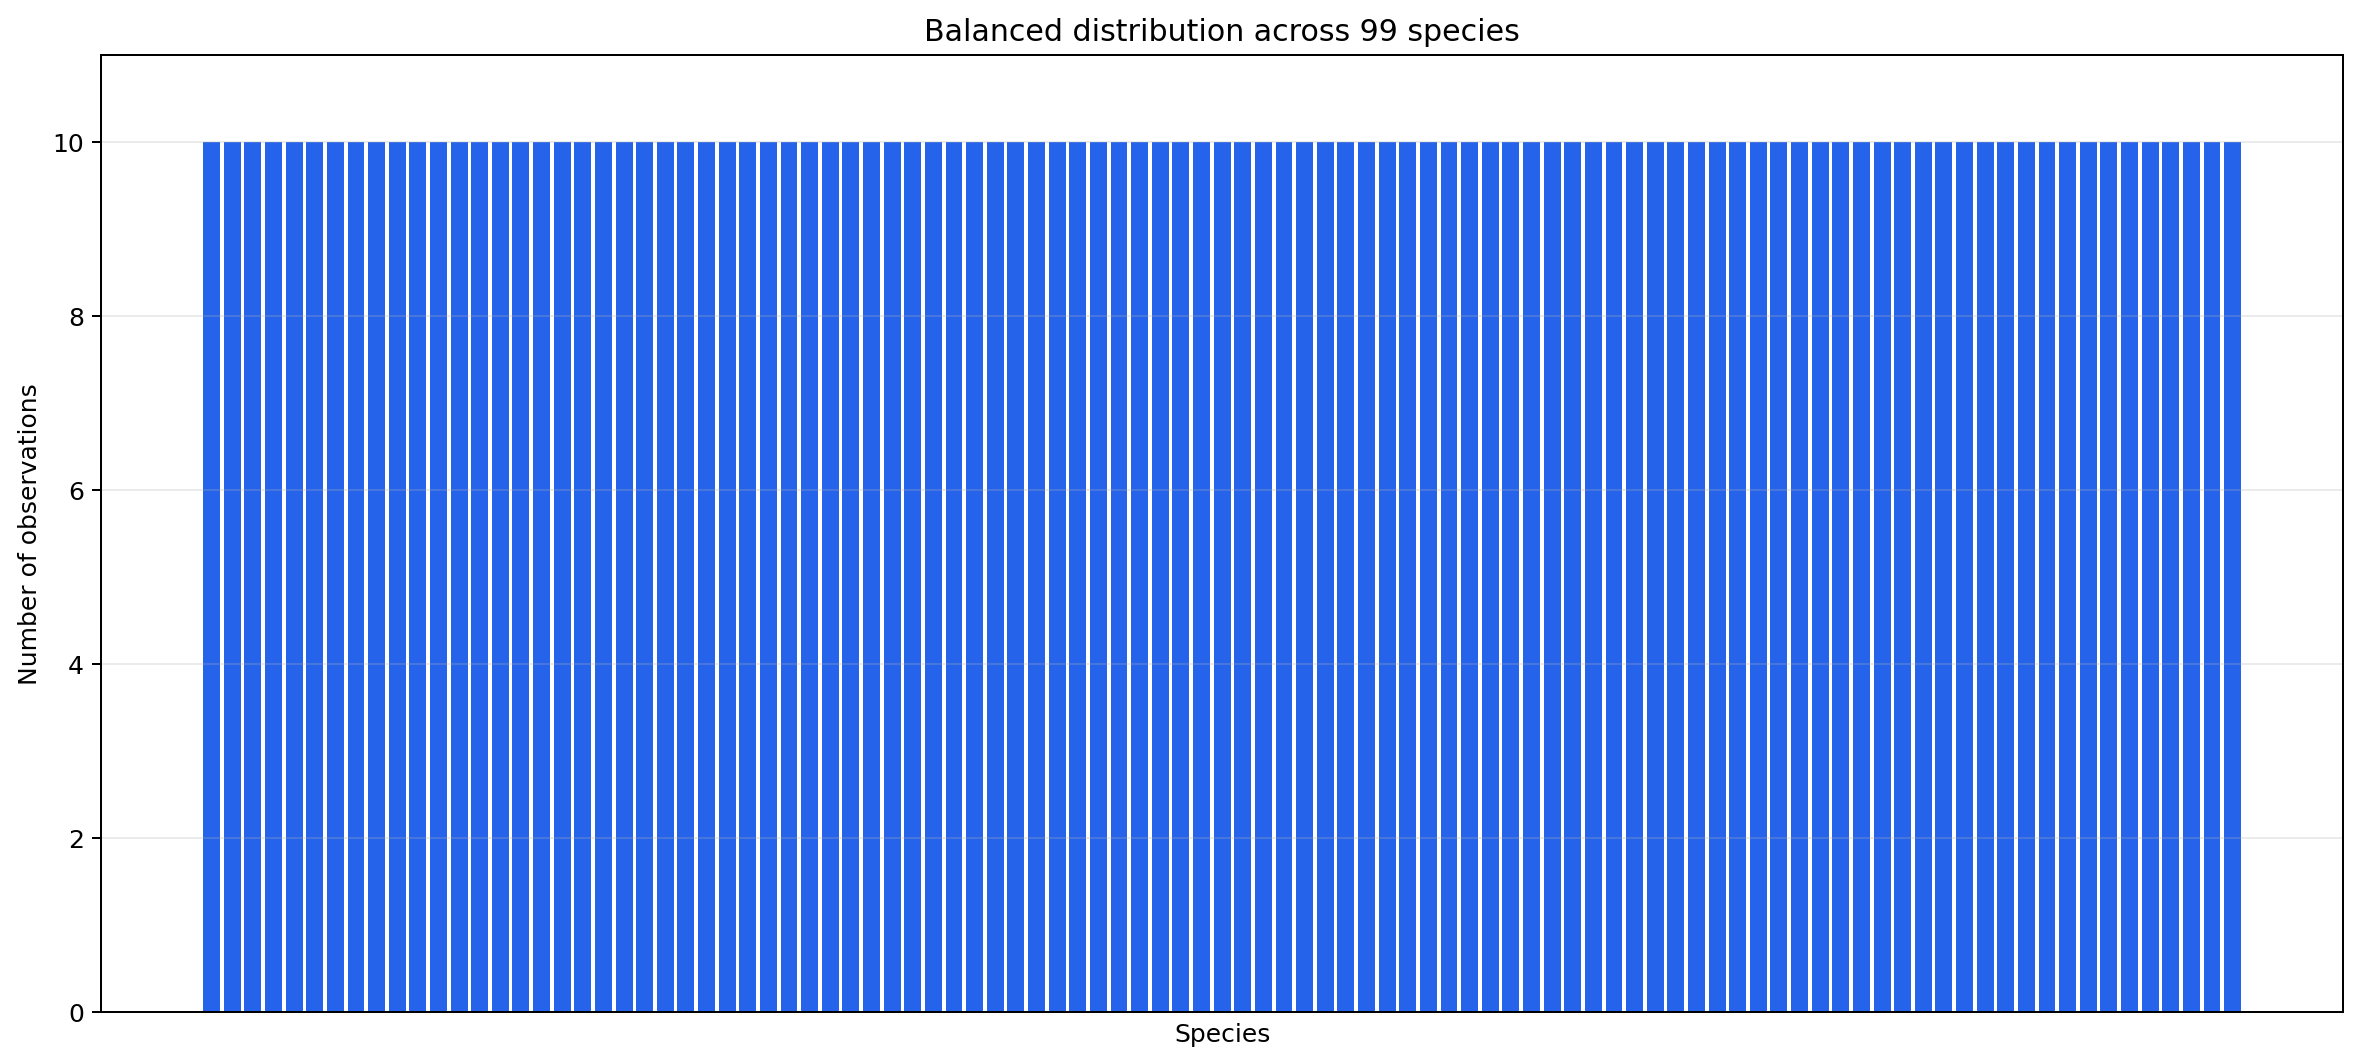
\includegraphics[width=\textwidth]{../figures/en/fig01_distribution_classes.png}
\caption{Number of observations per species. The uniform bar heights confirm that the training sample has no class imbalance.}
\end{figure}

\subsection{Feature scale, dispersion, and distributional shape}
The marginal distributions show that the three feature families operate on different scales. The \texttt{shape} variables occupy a very narrow range, with a mean standard deviation of \texttt{0.00029}, whereas the \texttt{margin} and \texttt{texture} variables have mean standard deviations of \texttt{0.01688} and \texttt{0.02696}, respectively. This scale heterogeneity is scientifically important because it directly affects methods that are sensitive to feature norms or to the geometry of the point cloud.

Boxplots play a central role here. Unlike a simple table of means, they simultaneously show the median, interquartile spread, skewness, and extreme values. In this dataset, they indicate that the \texttt{texture} family has the greatest dispersion, whereas \texttt{shape} is much more tightly concentrated. This observation does not establish that standardization will necessarily improve every learning procedure, but it provides a strong descriptive rationale for examining scaled variants.

\begin{table}[H]
\centering
\small
\begin{tabular}{|l|r|r|r|r|r|r|r|}
\hline
\textbf{Family} & \textbf{Min} & \textbf{Max} & \textbf{Mean Q1} & \textbf{Mean median} & \textbf{Mean Q3} & \textbf{Mean of means} & \textbf{Mean std. dev.} \\
\hline
\texttt{margin} & \texttt{0.00000} & \texttt{0.38867} & \texttt{0.00354} & \texttt{0.01028} & \texttt{0.02237} & \texttt{0.01562} & \texttt{0.01688} \\
\texttt{shape} & \texttt{0.00002} & \texttt{0.00301} & \texttt{0.00041} & \texttt{0.00056} & \texttt{0.00073} & \texttt{0.00061} & \texttt{0.00029} \\
\texttt{texture} & \texttt{0.00000} & \texttt{0.85352} & \texttt{0.00072} & \texttt{0.00543} & \texttt{0.01871} & \texttt{0.01563} & \texttt{0.02696} \\
\hline
\end{tabular}
\caption{Descriptive statistics by feature family}
\end{table}

\begin{figure}[H]
\centering
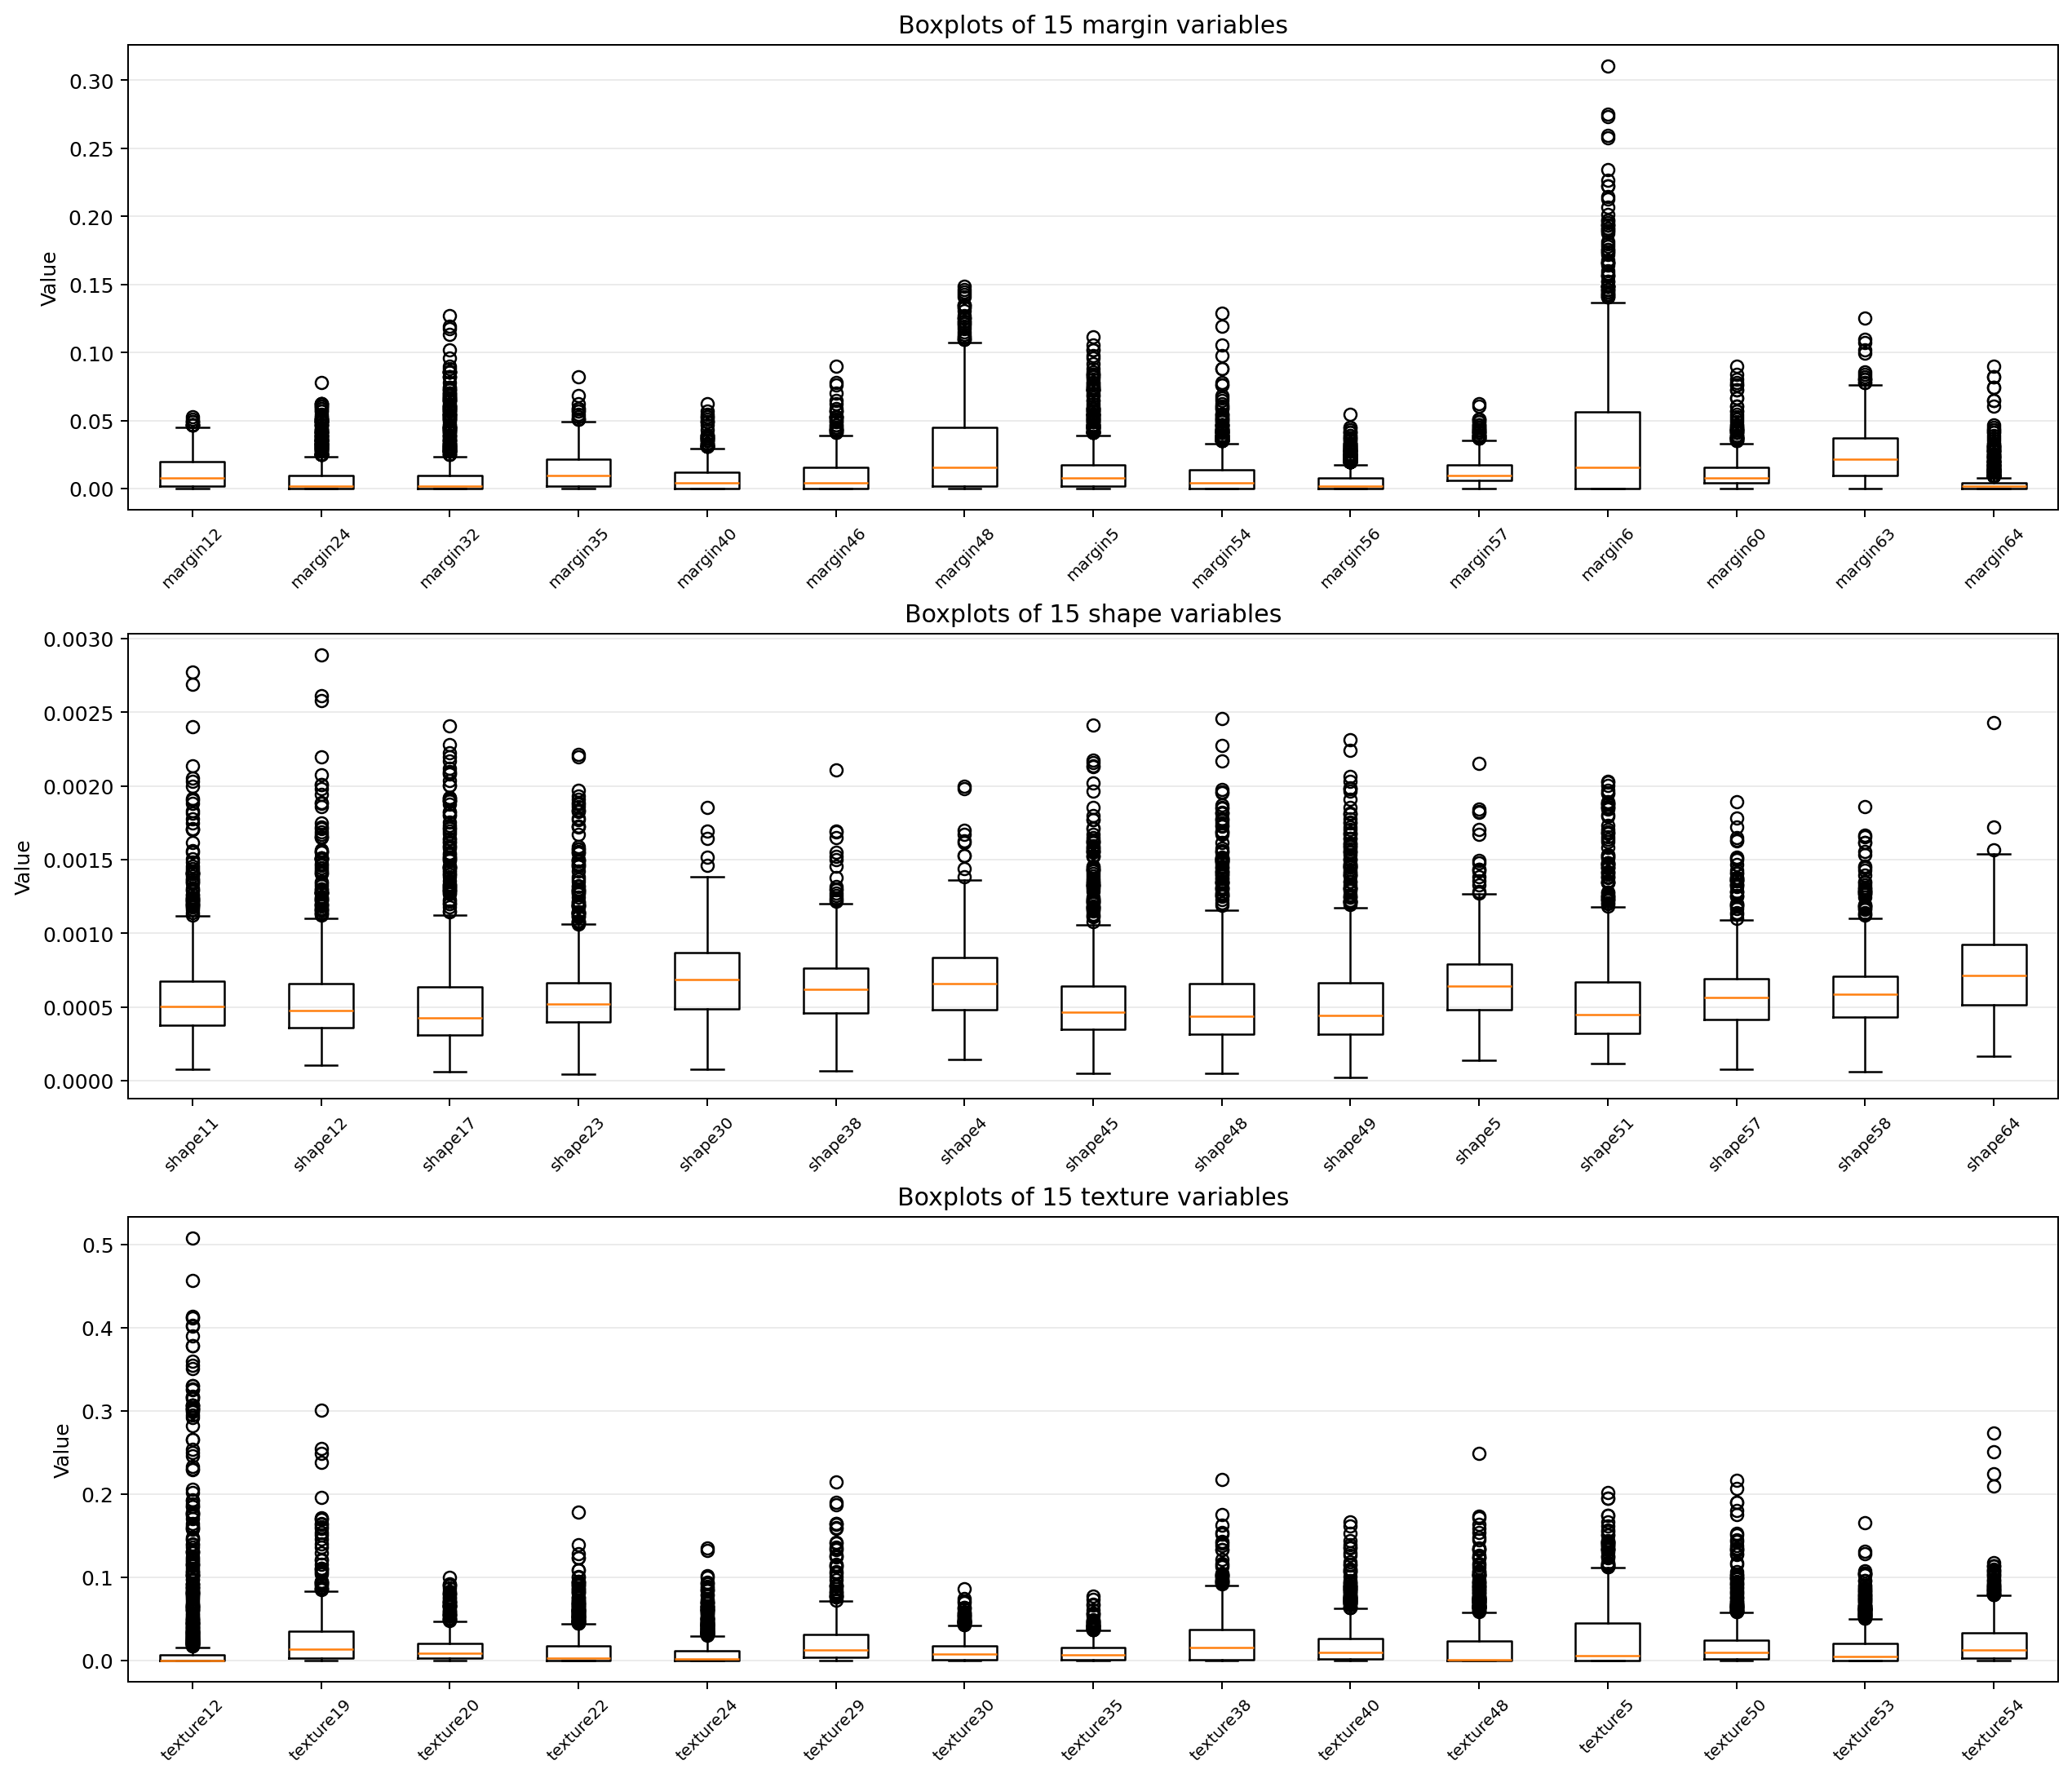
\includegraphics[width=\textwidth]{../figures/en/figA11_boxplots_variables.png}
\caption{Boxplots of selected variables from the \texttt{margin}, \texttt{shape}, and \texttt{texture} families. The visual comparison highlights scale heterogeneity and the greater dispersion of the texture variables.}
\end{figure}

The shape of the distributions supports this interpretation. The mean absolute skewness of the \texttt{192} variables is approximately \texttt{2.20}, with a maximum close to \texttt{10.91}, indicating distributions that are often asymmetric and sometimes strongly concentrated near zero. This result calls for caution when interpreting mean-based statistics alone and reinforces the value of robust descriptions based on quartiles and boxplots.

\subsection{Correlations and redundancy among descriptors}
The correlation matrix reveals a clear block structure. The \texttt{shape} family is by far the most redundant, with a mean absolute within-family correlation of \texttt{0.6996}, compared with \texttt{0.2606} for \texttt{margin} and \texttt{0.1612} for \texttt{texture}. Between-family dependencies remain weak, ranging from \texttt{0.0548} to \texttt{0.0781}, suggesting that the three families do not capture exactly the same descriptive information.

\begin{table}[H]
\centering
\begin{tabular}{|l|r|}
\hline
\textbf{Block} & \textbf{Mean absolute correlation} \\
\hline
\texttt{shape-shape} & \texttt{0.6996} \\
\texttt{margin-margin} & \texttt{0.2606} \\
\texttt{texture-texture} & \texttt{0.1612} \\
\texttt{margin-shape} & \texttt{0.0675} \\
\texttt{margin-texture} & \texttt{0.0781} \\
\texttt{shape-texture} & \texttt{0.0548} \\
\hline
\end{tabular}
\caption{Mean absolute within- and between-family correlation}
\end{table}

\begin{table}[H]
\centering
\begin{tabular}{|c|l|r|}
\hline
\textbf{Rank} & \textbf{Pair} & \textbf{Correlation} \\
\hline
1 & \texttt{shape49} - \texttt{shape50} & \texttt{0.9939} \\
2 & \texttt{shape17} - \texttt{shape18} & \texttt{0.9939} \\
3 & \texttt{shape15} - \texttt{shape16} & \texttt{0.9937} \\
4 & \texttt{shape16} - \texttt{shape17} & \texttt{0.9936} \\
5 & \texttt{shape18} - \texttt{shape19} & \texttt{0.9936} \\
\hline
\end{tabular}
\caption{Most highly correlated variable pairs}
\end{table}

In total, \texttt{445} variable pairs have an absolute correlation of at least \texttt{0.90}, and \texttt{197} have a correlation of at least \texttt{0.95}. These magnitudes justify examining dimensionality reduction with \texttt{PCA}, without presuming that it will benefit the subsequent learning stages.

\begin{figure}[H]
\centering
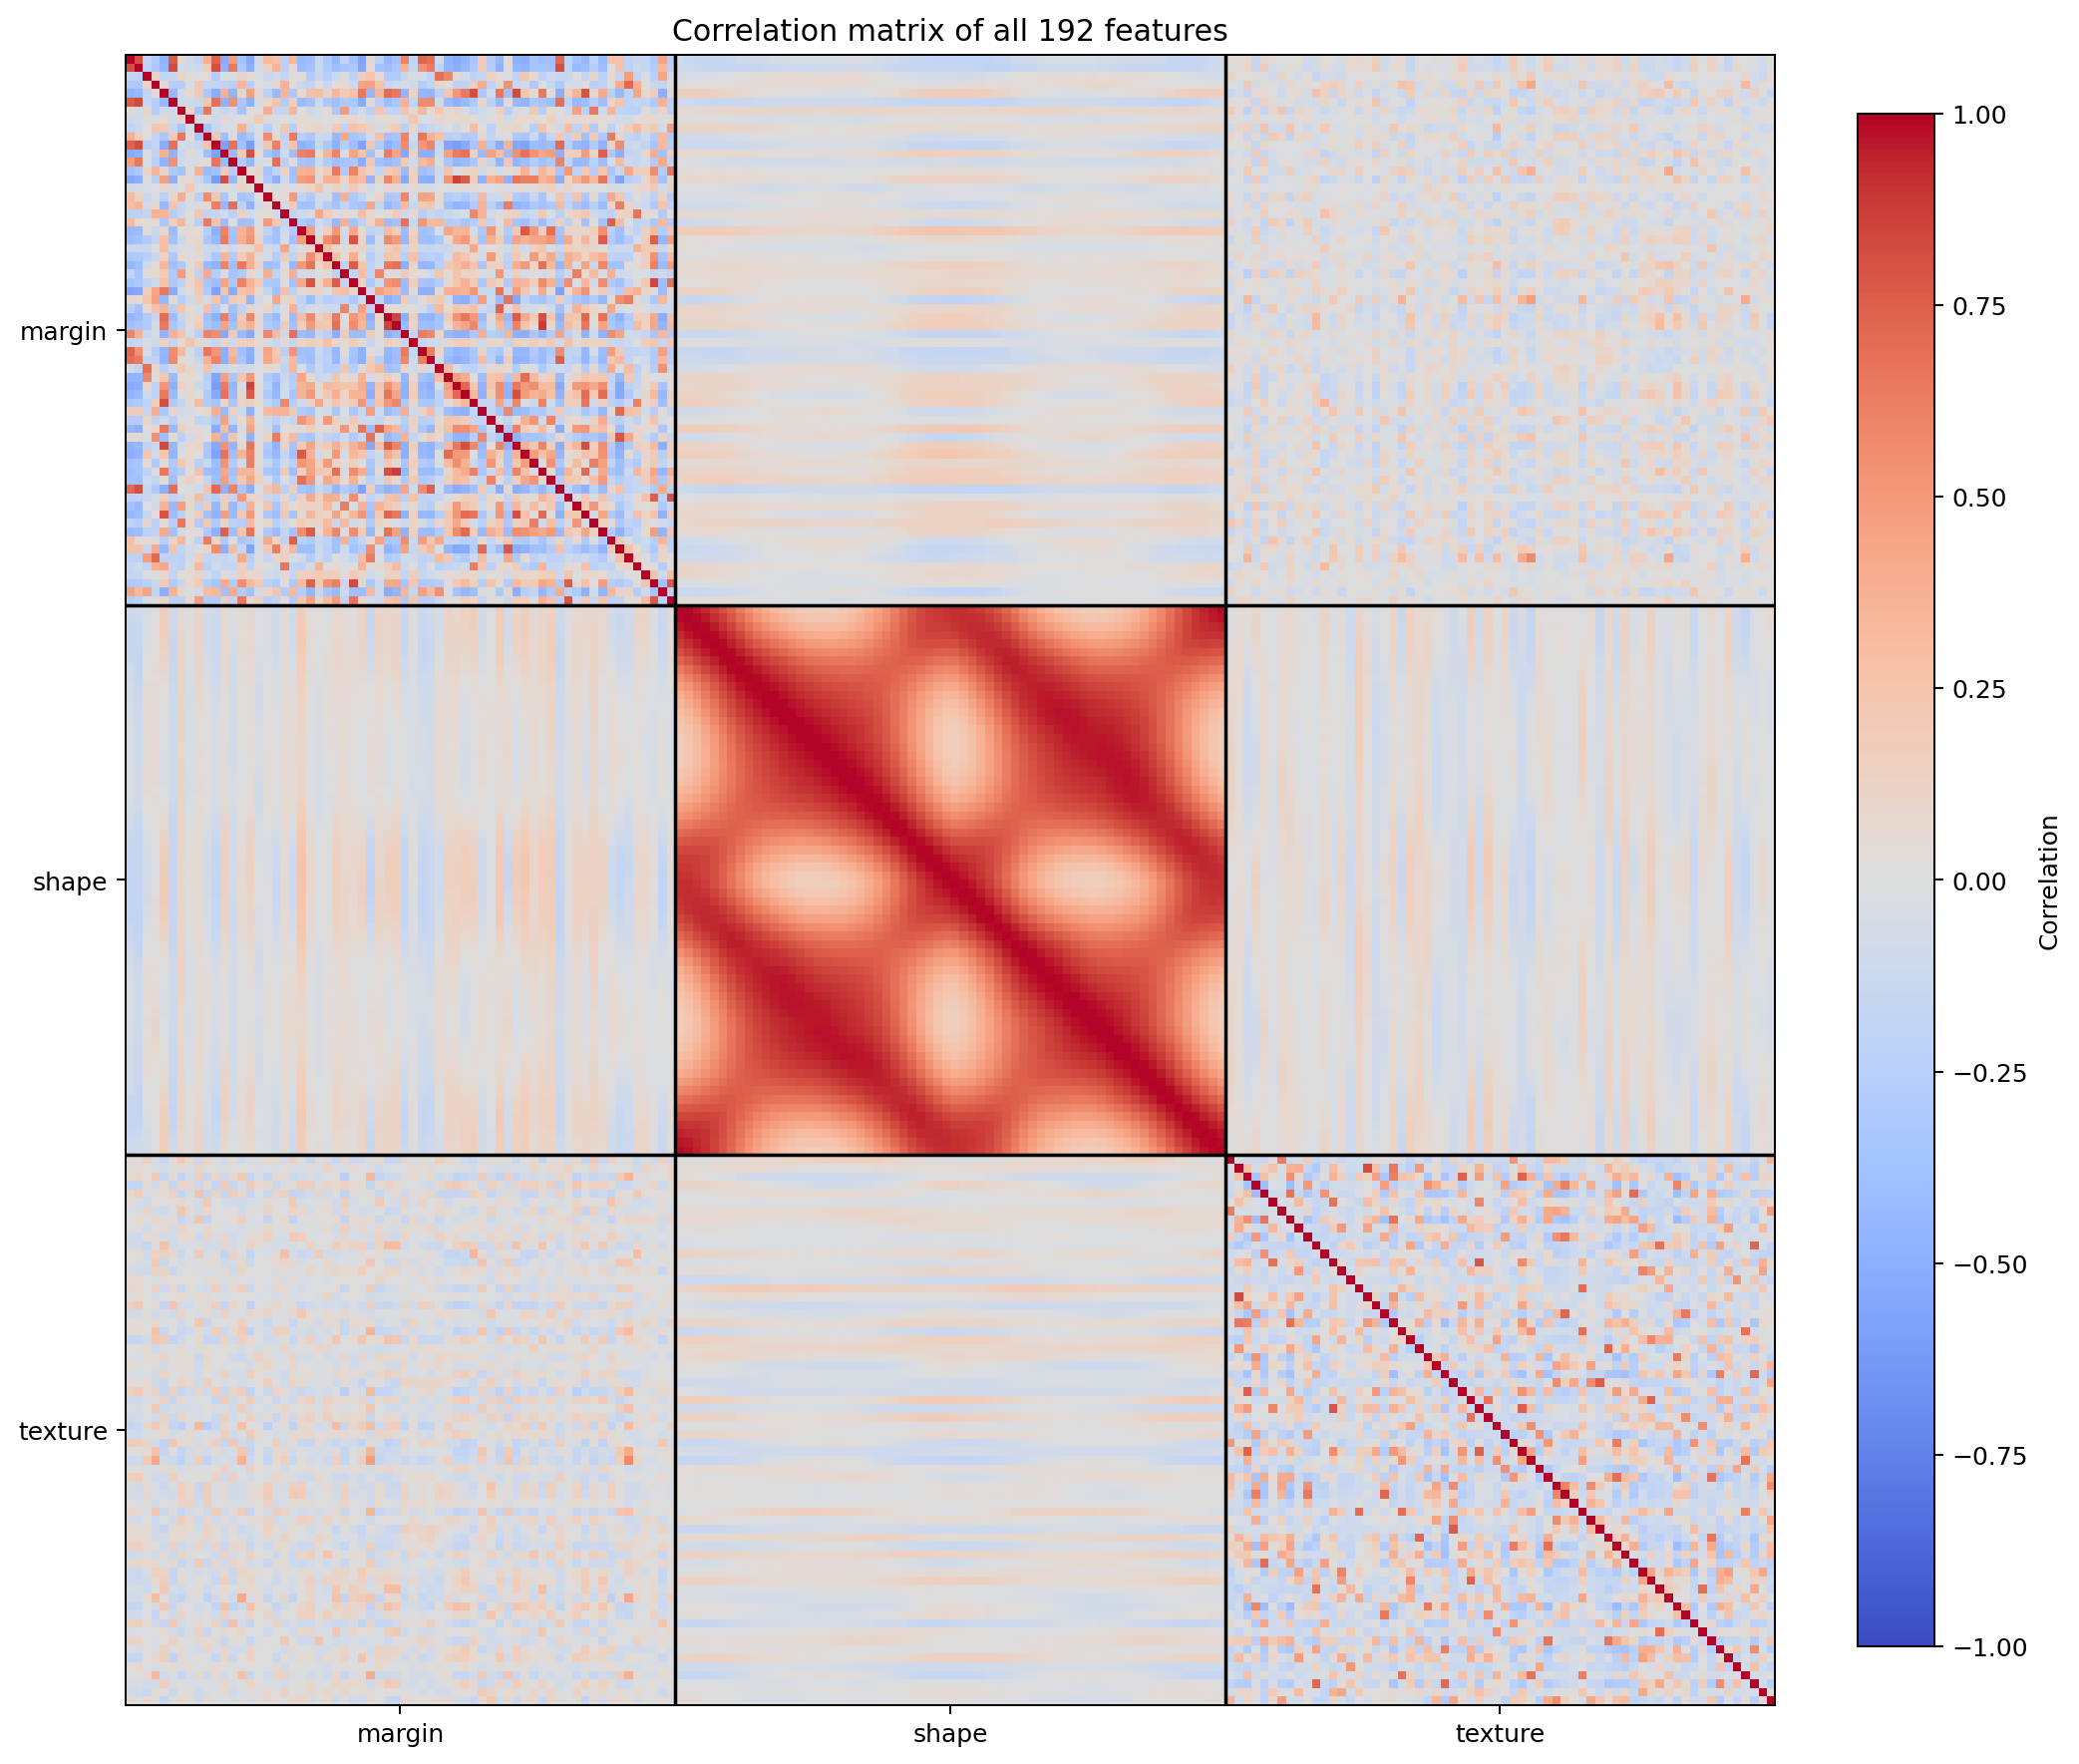
\includegraphics[width=\textwidth]{../figures/en/figA12_heatmap_correlation.png}
\caption{Correlation matrix for the \texttt{192} variables. The block structure reveals particularly strong internal redundancy within the \texttt{shape} family, while relationships between families remain weaker.}
\end{figure}

\subsection{Dimensionality reduction and global organization}
\texttt{PCA} was applied to the standardized data to summarize the dataset's linear structure. The first two components explain approximately \texttt{24.2 \%} and \texttt{10.4 \%} of the total variance, or just under \texttt{34.6 \%} combined. The first five components account for \texttt{50.7 \%}, and the first ten for \texttt{64.7 \%}. The reduction is therefore meaningful, but not radical enough to suggest that a very low-dimensional space would adequately summarize the information.

The cumulative variance thresholds reinforce this interpretation. It takes \texttt{23} components to reach \texttt{80 \%} explained variance, \texttt{44} to reach \texttt{90 \%}, \texttt{69} to reach \texttt{95 \%}, and \texttt{116} to reach \texttt{99 \%}. Thus, \texttt{PCA} is defensible as a tool for moderate compression and mitigation of linear redundancy, but not as a drastic reduction of the problem.

\begin{table}[H]
\centering
\begin{tabular}{|l|r|}
\hline
\textbf{Cumulative explained variance} & \textbf{Number of components} \\
\hline
\texttt{80 \%} & \texttt{23} \\
\texttt{90 \%} & \texttt{44} \\
\texttt{95 \%} & \texttt{69} \\
\texttt{99 \%} & \texttt{116} \\
\hline
\end{tabular}
\caption{Number of components required at different variance thresholds}
\end{table}

\begin{figure}[H]
\centering
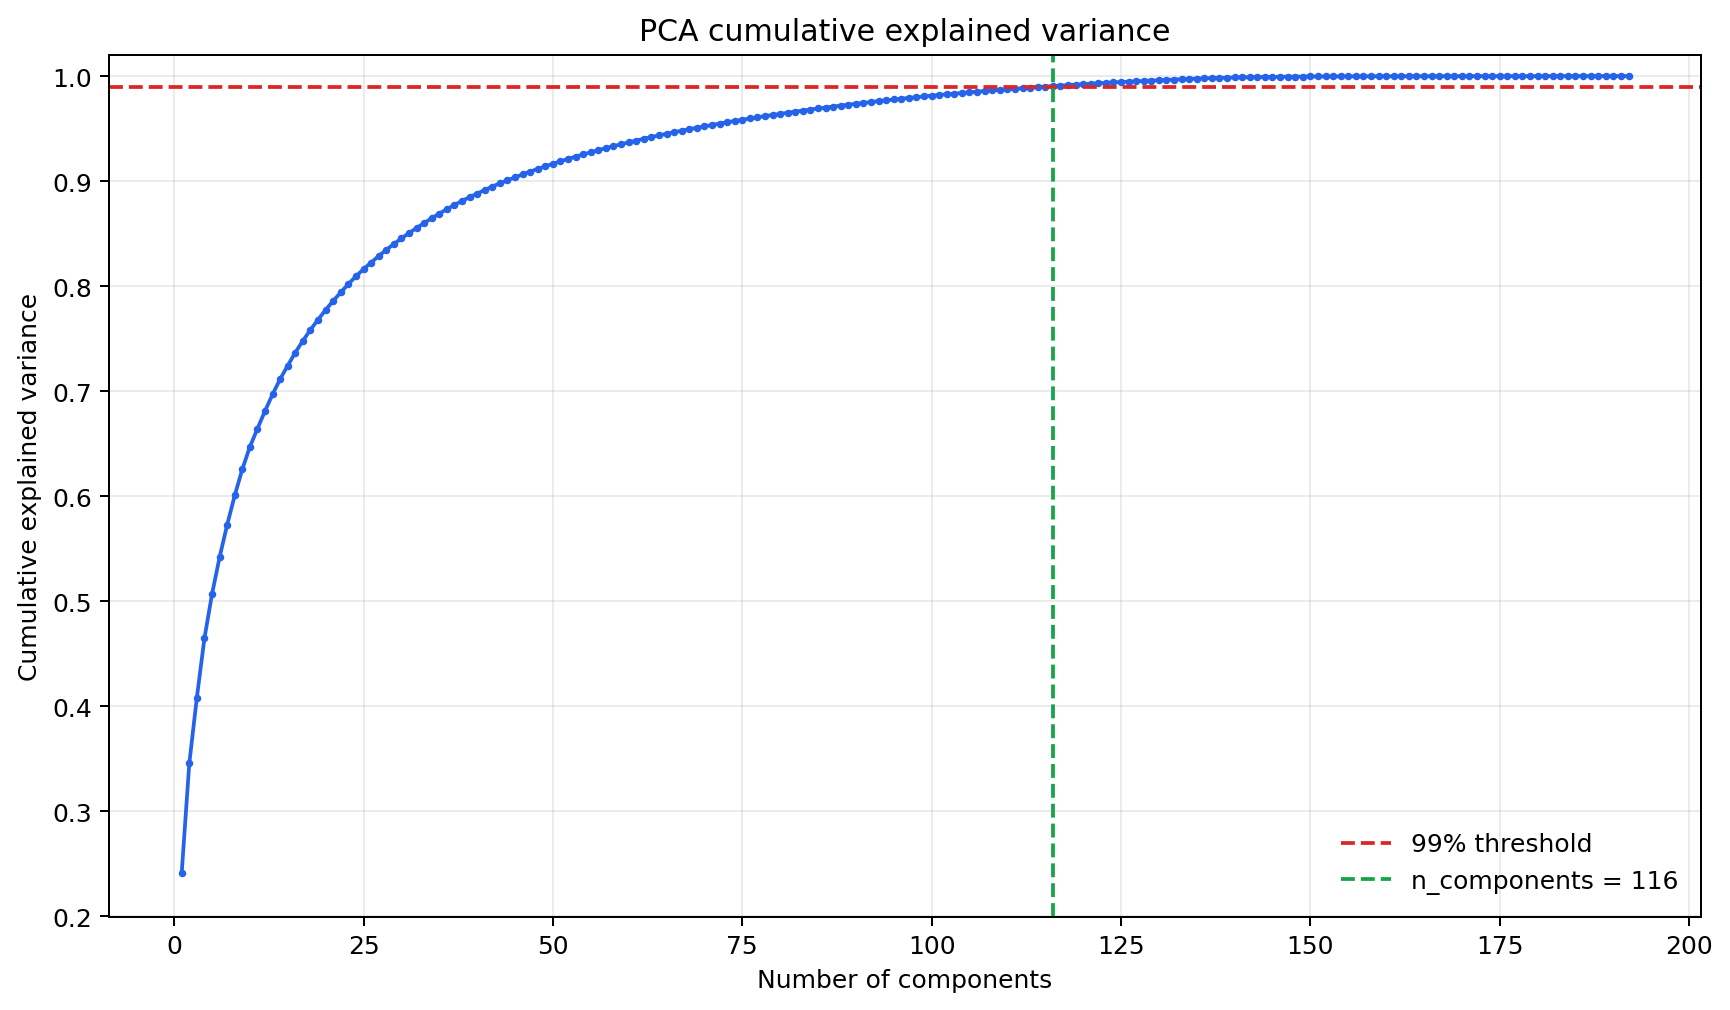
\includegraphics[width=\textwidth]{../figures/en/figA13_pca_variance_cumulative.png}
\caption{Cumulative explained variance after standardization. The curve's gradual increase indicates that much of the information can be compressed, but that a substantial number of components is still required to retain nearly all variance.}
\end{figure}

The two-dimensional \texttt{t-SNE} projection complements this linear view. In the notebook, it is computed after an initial \texttt{PCA} reduction to \texttt{50} components, with a perplexity of \texttt{30}. Its purpose is not to summarize variance quantitatively, but to examine the local consistency of neighborhoods among observations. The figure reveals partial groupings alongside overlapping regions, suggesting exploitable structure without implying trivial separation of the \texttt{99} species in a very low-dimensional space.

This interpretation must remain cautious. \texttt{t-SNE} primarily preserves local proximity relationships and depends on its hyperparameters; it provides neither a measure of global separability nor sufficient evidence to favor a particular preprocessing method. Its value here is heuristic: it confirms organization in the point cloud beyond pure noise without establishing the exact difficulty of the task.

\begin{figure}[H]
\centering
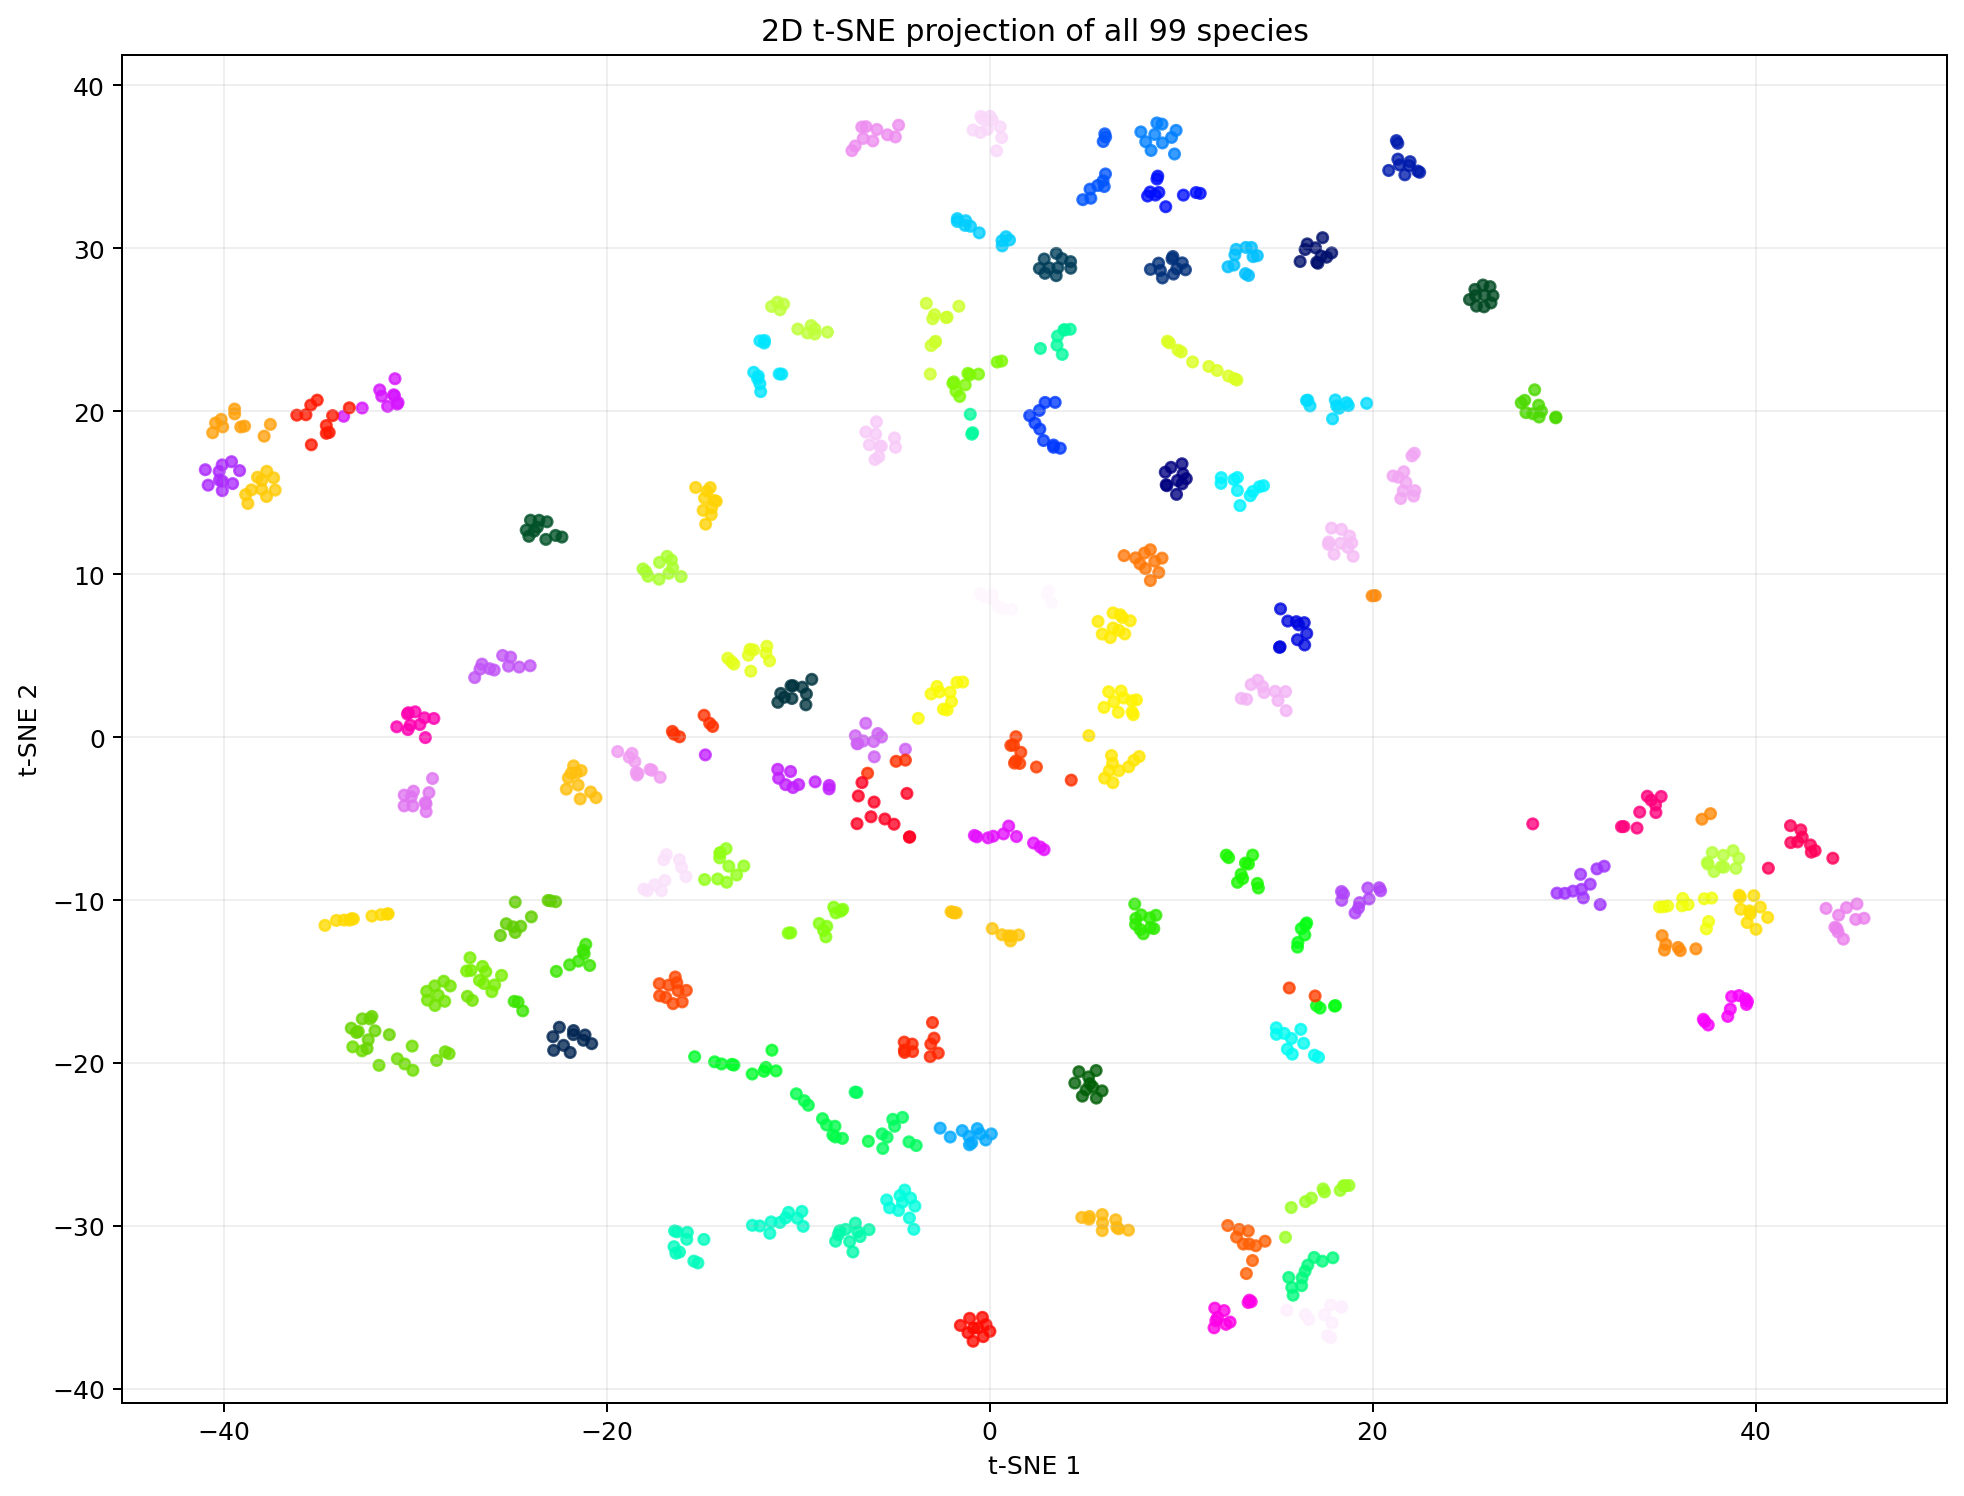
\includegraphics[width=\textwidth]{../figures/en/figA14_tsne_2d.png}
\caption{\texttt{t-SNE} 2D projection of the \texttt{99} species after standardization and an initial \texttt{PCA} reduction. Local clusters coexist with substantial overlap, consistent with a learnable problem that is far from trivial.}
\end{figure}

\subsection{Methodological implications and summary}
Four lessons emerge from this exploratory analysis. First, the dataset is structurally sound and perfectly balanced, but remains sparse at the species level, calling for restraint when interpreting variations observed on small subsets. Second, the differences in scale and dispersion among feature families provide a strong descriptive motivation for examining standardization procedures. Third, the pronounced redundancy, especially within \texttt{shape}, makes the study of \texttt{PCA} as a linear compression method methodologically plausible. Fourth, the reduced-dimensional projections indicate exploitable structure while emphasizing that this structure is not equivalent to simple separability.

Consequently, the preprocessing choices examined later can be scientifically motivated by this EDA, but they remain hypotheses at this stage. Standardization and \texttt{PCA} are reasonable exploratory options, not guarantees of improvement.

\subsection{Protocol safeguards for the subsequent analysis}
The preceding descriptive findings justify a cautious protocol for model comparison. The dataset is balanced, but each species remains sparsely represented; it would therefore be methodologically risky to combine variant selection, tuning, and final evaluation on the same subset. For this reason, the remainder of the report explicitly distinguishes exploration, confirmation, and secondary corroboration.

\begin{table}[H]
\centering
\begin{tabular}{|l|l|}
\hline
\textbf{Element} & \textbf{Selected value} \\
\hline
Frozen split & \texttt{80 \%} development / \texttt{20 \%} corroboration \\
Development-set size & \texttt{792} \\
Corroboration-set size & \texttt{198} \\
Primary cross-validation & \texttt{5} outer folds \\
Inner tuning & \texttt{3} inner folds \\
Primary metric & \texttt{F1-macro} \\
Secondary metric & \texttt{Accuracy} \\
Global seed & \texttt{42} \\
Status of non-\texttt{tuned} variants & \texttt{Exploratory} \\
Status of \texttt{tuned} variants & \texttt{Confirmatory} \\
Status of corroboration set & \texttt{Secondary corroboration} \\
\hline
\end{tabular}
\caption{Safeguards in the experimental protocol}
\end{table}

This evidence hierarchy guides the reading of all subsequent sections. The non-\texttt{tuned} variants document the effects of preprocessing and tuning, the \texttt{tuned} results determine the primary ranking, and the frozen corroboration set is used only for secondary verification.

% ==========================================
% 3. MODEL STUDY
% ==========================================
